%%% research_paper.tex
%%% Publication-quality research paper on the kissing number in dimension 5
%%% via dimensional analysis on calculus

\documentclass[11pt,a4paper]{article}

% ---------- Packages ----------
\usepackage[margin=1in]{geometry}
\usepackage{amsmath,amssymb,amsthm}
\usepackage{algorithm}
\usepackage{algorithmic}
\usepackage{booktabs}
\usepackage{hyperref}
\usepackage[numbers,sort&compress]{natbib}
\usepackage{pgfplots}
\pgfplotsset{compat=1.18}
\usepackage{tikz}
\usetikzlibrary{arrows.meta,positioning,calc,decorations.pathreplacing,shapes.geometric}
\usepackage{subcaption}
\usepackage{multirow}
\usepackage{xcolor}
\usepackage{graphicx}
\usepackage{enumitem}
\usepackage{microtype}

% ---------- Theorem environments ----------
\newtheorem{theorem}{Theorem}[section]
\newtheorem{lemma}[theorem]{Lemma}
\newtheorem{proposition}[theorem]{Proposition}
\newtheorem{corollary}[theorem]{Corollary}
\theoremstyle{definition}
\newtheorem{definition}[theorem]{Definition}
\theoremstyle{remark}
\newtheorem{remark}[theorem]{Remark}

% ---------- Custom commands ----------
\newcommand{\R}{\mathbb{R}}
\newcommand{\Sn}[1]{S^{#1}}
\newcommand{\caparea}{A_{\mathrm{cap}}}
\newcommand{\Vn}{V_n}
\newcommand{\Ssurf}{S_{n-1}}
\DeclareMathOperator{\tr}{tr}

% ---------- Title ----------
\title{\textbf{The Kissing Number in Dimension Five:\\
Dimensional Analysis on Calculus, Pyramid Decomposition,\\
and the Limits of Geometric Bounding Methods}}

\author{Research Lab (Automated)}
\date{February 2026}

% ==========================================================================
\begin{document}
\maketitle

% ---------- Abstract ----------
\begin{abstract}
The kissing number $\tau_5$ in $\R^5$---the maximum number of non-overlapping
unit spheres that can simultaneously touch a central unit sphere---is one of
the longest-standing open problems in discrete geometry, with the best known
bounds $40\le\tau_5\le 44$.  We investigate whether the \emph{dimensional
analysis on calculus} framework, rooted in the derivative relation
$\frac{d}{dR}[V_n(R)]=S_{n-1}(R)$, the two-step volume recurrence
$V_n=\frac{2\pi}{n}R^{2}V_{n-2}$, and the pyramid decomposition
$V_n=\frac{1}{n}R\,S_{n-1}$, can produce improved bounds.  We implement the
Delsarte linear programming bound augmented with three dimensional integration
constraints (equatorial slicing, Gram matrix trace, volume recurrence
consistency), perform contact graph analysis with a refined vertex degree bound
of~21 (improved from the na\"ive bound of~24), and carry out extensive
computational searches for a 41-point kissing configuration.  Our principal
finding is a carefully documented negative result: the dimensional constraints
are redundant within the Delsarte LP framework, and no improved bound or
construction was obtained.  Nevertheless, the investigation yields novel
geometric insights---including an elementary proof of local rigidity for the
$D_5$ configuration with angular gap $9.23^\circ$, a refined contact graph
degree bound $d(v)\le 21$, and a systematic cap density analysis---that
clarify the boundary between geometric and spectral methods for bounding
kissing numbers.
\end{abstract}

% ---------- 1. Introduction ----------
\section{Introduction}\label{sec:intro}

The kissing number problem asks: in $n$-dimensional Euclidean space, what is
the maximum number of non-overlapping unit spheres that can simultaneously be
tangent to a central unit sphere?  This maximum, denoted $\tau_n$, is
equivalently the largest cardinality of a set of unit vectors on $\Sn{n-1}$
with pairwise angular separation at least $60^\circ$.  The problem has a rich
history stretching back to the Newton--Gregory debate of 1694, and the exact
value of $\tau_n$ is known in only six dimensions:
$\tau_1=2$, $\tau_2=6$, $\tau_3=12$~\cite{schutte1953problem},
$\tau_4=24$~\cite{musin2008kissing},
$\tau_8=240$, and $\tau_{24}=196\,560$~\cite{odlyzko1979kissing}.

Dimension five is the first open case.  The best known bounds are
\begin{equation}\label{eq:gap}
  40 \;\le\; \tau_5 \;\le\; 44,
\end{equation}
where the lower bound is achieved by the $D_5$ root lattice~\cite{conway1999sphere}
and the upper bound is due to the high-accuracy semidefinite programming (SDP)
computation of Mittelmann and Vallentin~\cite{mittelmann2010high}, building on
the framework of Bachoc and Vallentin~\cite{bachoc2008new}.

\paragraph{Motivation.}
The \emph{dimensional analysis on calculus} framework starts from the elementary
observation that $\frac{d}{dx}[x^2]=2x$ encodes the fact that a square is
bounded by two lines, and $\int x^2\,dx = x^3/3$ encodes the fact that a
square-base pyramid has volume one-third of its bounding cube.  Extending this
to $n$~dimensions, the derivative relation $\frac{d}{dR}[V_n(R)]=S_{n-1}(R)$,
the two-step recurrence $V_n=\frac{2\pi}{n}R^2 V_{n-2}$, and the pyramid
identity $V_n=\frac{1}{n}R\,S_{n-1}$ create a web of cross-dimensional
constraints.  We ask: can these constraints, when combined with the Delsarte
linear programming framework, tighten the upper bound on~$\tau_5$?

\paragraph{Contributions.}
Our investigation produces the following results:
\begin{enumerate}[label=(\arabic*)]
  \item A complete formalization of the dimensional analysis framework applied
        to spherical cap packing on~$\Sn{4}$, including cap area computation
        via the regularized incomplete beta function (Section~\ref{sec:method}).
  \item An enhanced Delsarte LP augmented with three dimensional integration
        constraints (D1--D3), with a thorough sensitivity analysis demonstrating
        that all three are redundant for $n=5$ (Section~\ref{sec:results}).
  \item A refined contact graph degree bound $d(v)\le 21$ for kissing
        configurations in $\R^5$, improved from the na\"ive $\tau_4=24$
        (Theorem~\ref{thm:degree}).
  \item An elementary proof that the $D_5$ configuration is locally rigid
        against augmentation, with minimum maximum inner product
        $\sqrt{2/5}\approx 0.6325$ and angular gap $9.23^\circ$
        (Theorem~\ref{thm:rigidity}).
  \item A systematic cap density analysis across dimensions $2$--$24$, showing
        that $\rho_5\in[0.514,0.566]$ for $\tau_5\in[40,44]$
        (Section~\ref{sec:pyramid}).
  \item A comprehensive comparison with 16~papers from the literature,
        documenting an honest negative result: the dimensional analysis
        framework does not improve bounds beyond the known
        $\tau_5\le 44$ (Section~\ref{sec:discussion}).
  \item Independent numerical verification of all results at up to 128-digit
        precision using \texttt{mpmath} (Section~\ref{sec:verification}).
\end{enumerate}

\paragraph{Paper outline.}
Section~\ref{sec:related} surveys related work.
Section~\ref{sec:background} establishes notation and key identities.
Section~\ref{sec:method} describes our methods.
Section~\ref{sec:setup} details the experimental setup.
Section~\ref{sec:results} presents results.
Section~\ref{sec:discussion} discusses implications and limitations.
Section~\ref{sec:conclusion} concludes.

% ---------- 2. Related Work ----------
\section{Related Work}\label{sec:related}

\paragraph{Classical bounds.}
The Delsarte linear programming method~\cite{delsarte1973algebraic,delsarte1977spherical},
systematically applied by Odlyzko and Sloane~\cite{odlyzko1979kissing} and
Levenshtein~\cite{levenshtein1979boundaries}, yields $\tau_5\le 46$ using
optimal Gegenbauer polynomial certificates.  The asymptotic bounds of
Kabatyansky and Levenshtein~\cite{kabatyansky1978bounds} give
$\tau_n\le 2^{0.401n(1+o(1))}$ but are not sharp for specific small dimensions.
Pfender~\cite{pfender2007improved} refined the Delsarte bounds for small dimensions.

\paragraph{Semidefinite programming.}
Bachoc and Vallentin~\cite{bachoc2008new} introduced SDP bounds incorporating
three-point correlations, improving $\tau_5\le 45$.  Mittelmann and
Vallentin~\cite{mittelmann2010high} performed high-accuracy SDP to obtain
$\tau_5\le 44$.  Machado and de~Oliveira Filho~\cite{machado2018improving}
exploited polynomial symmetry to further refine SDP bounds.

\paragraph{Lattice constructions and lower bounds.}
The $D_5$ root lattice yields 40~kissing vectors~\cite{conway1999sphere}.
Sz\"oll\H{o}si~\cite{szollosi2023five} discovered a third non-isometric 40-point
arrangement~$Q_5$, and Cohn and Rajagopal~\cite{cohn2024variations} subsequently
constructed a fourth.  No 41-point configuration has ever been found.

\paragraph{Special dimensions and modular forms.}
The cases $n=8$ and $n=24$ were resolved using ``magic'' polynomials matching
the inner product spectra of $E_8$ and the Leech lattice~\cite{odlyzko1979kissing}.
Viazovska's proof of optimal sphere packing in dimension~8~\cite{viazovska2017sphere}
and the Cohn--Elkies linear programming approach~\cite{cohn2003new} demonstrated
the power of modular form techniques, though these currently apply only in
dimensions~8 and~24.  Cohn and Kumar~\cite{cohn2007universally} established
universal optimality results for certain spherical codes.

\paragraph{Surveys.}
The surveys of Pfender and Ziegler~\cite{pfender2004kissing},
Boyvalenkov \emph{et al.}~\cite{boyvalenkov2012survey}, and
Zong~\cite{zong2008kissing} provide comprehensive overviews of the field.

% ---------- 3. Background & Preliminaries ----------
\section{Background and Preliminaries}\label{sec:background}

\subsection{Notation}

Table~\ref{tab:notation} summarizes the key notation used throughout.

\begin{table}[ht]
  \centering
  \caption{Notation table.}\label{tab:notation}
  \begin{tabular}{@{}ll@{}}
    \toprule
    Symbol & Meaning \\
    \midrule
    $\tau_n$ & Kissing number in $\R^n$ \\
    $V_n(R)$ & Volume of the $n$-dimensional ball of radius $R$ \\
    $S_{n-1}(R)$ & Surface area of $\Sn{n-1}(R)$ \\
    $\caparea(n,\theta)$ & Area of a spherical cap of half-angle $\theta$ on $\Sn{n-1}$ \\
    $\omega(n,\theta)$ & Fractional solid angle: $\caparea(n,\theta)/S_{n-1}(1)$ \\
    $\rho_n$ & Cap density: $\tau_n\cdot\omega(n,\pi/6)$ \\
    $I_x(a,b)$ & Regularized incomplete beta function \\
    $C_k^{(\lambda)}(t)$ & Gegenbauer polynomial with $\lambda=(n-2)/2$ \\
    $D_5$ & Root lattice in $\R^5$ with minimal vectors $(\pm 1,\pm 1,0,0,0)/\!\sqrt{2}$ \\
    \bottomrule
  \end{tabular}
\end{table}

\subsection{Volume and Surface Area of the $n$-Ball}

The volume and surface area of the unit $n$-ball are
\begin{equation}\label{eq:volume}
  V_n(R) = \frac{\pi^{n/2}}{\Gamma(n/2+1)}\,R^n,
  \qquad
  S_{n-1}(R) = \frac{2\pi^{n/2}}{\Gamma(n/2)}\,R^{n-1}.
\end{equation}
The fundamental derivative relationship is
\begin{equation}\label{eq:deriv}
  \frac{d}{dR}\bigl[V_n(R)\bigr] = S_{n-1}(R),
\end{equation}
and the two-step volume recurrence is
\begin{equation}\label{eq:recurrence}
  V_n(R) = \frac{2\pi}{n}\,R^2\,V_{n-2}(R).
\end{equation}

\subsection{The Pyramid Decomposition}\label{sec:pyramid-bg}

Decomposing the $n$-ball into infinitesimal cones radiating from the center,
each subtending solid angle $d\Omega$ on $\Sn{n-1}$, yields
\begin{equation}\label{eq:pyramid}
  dV = \frac{1}{n}\,R^n\,d\Omega,
  \qquad
  V_n(R) = \frac{1}{n}\,R\,S_{n-1}(R).
\end{equation}
This is the higher-dimensional analogue of the classical result
$\int_0^R r^2\,dr = R^3/3$: a three-dimensional cone fills one-third of its
bounding cylinder, and an $n$-dimensional cone fills~$1/n$.

\subsection{Spherical Cap Area}

The area of a spherical cap of half-angle~$\theta$ on $\Sn{n-1}$ is
\begin{equation}\label{eq:caparea}
  \caparea(n,\theta) = \frac{S_{n-1}(1)}{2}\;
    I_{\sin^2\!\theta}\!\Bigl(\frac{n-1}{2},\,\frac{1}{2}\Bigr),
\end{equation}
obtained by integrating lower-dimensional cross-sections:
\begin{equation}\label{eq:capintegral}
  \caparea(n,\theta) = \frac{2\pi^{(n-1)/2}}{\Gamma\!\bigl(\frac{n-1}{2}\bigr)}
    \int_0^{\theta} (\sin\phi)^{n-2}\,d\phi.
\end{equation}
For $n=5$ and $\theta=\pi/6$ (the kissing exclusion half-angle), numerical
evaluation gives $\caparea(5,\pi/6) = 0.3385$, verified to 50~decimal digits
via \texttt{mpmath}.

\subsection{The Delsarte Linear Programming Bound}

The Delsarte LP bound~\cite{delsarte1973algebraic,delsarte1977spherical} states
\begin{equation}\label{eq:delsarte}
  \tau_n \;\le\; \frac{f(1)}{f_0},
\end{equation}
for any polynomial $f(t)=\sum_{k=0}^{d}f_k\,C_k^{(\lambda)}(t)$ with
$\lambda=(n-2)/2$ satisfying:
\begin{enumerate}[label=(A\arabic*)]
  \item $f(t)\le 0$ for all $t\in[-1,\,1/2]$, and
  \item $f_k\ge 0$ for all $k\ge 1$ (non-negative Gegenbauer coefficients).
\end{enumerate}
This bound is tight for $n\in\{2,8,24\}$ due to the existence of
``magic'' polynomials whose roots match the inner product spectra of optimal
codes~\cite{odlyzko1979kissing}.

% ---------- 4. Method ----------
\section{Method}\label{sec:method}

Figure~\ref{fig:architecture} provides an overview of our methodology,
combining the dimensional analysis framework with the Delsarte LP and contact
graph analysis.

\begin{figure}[ht]
\centering
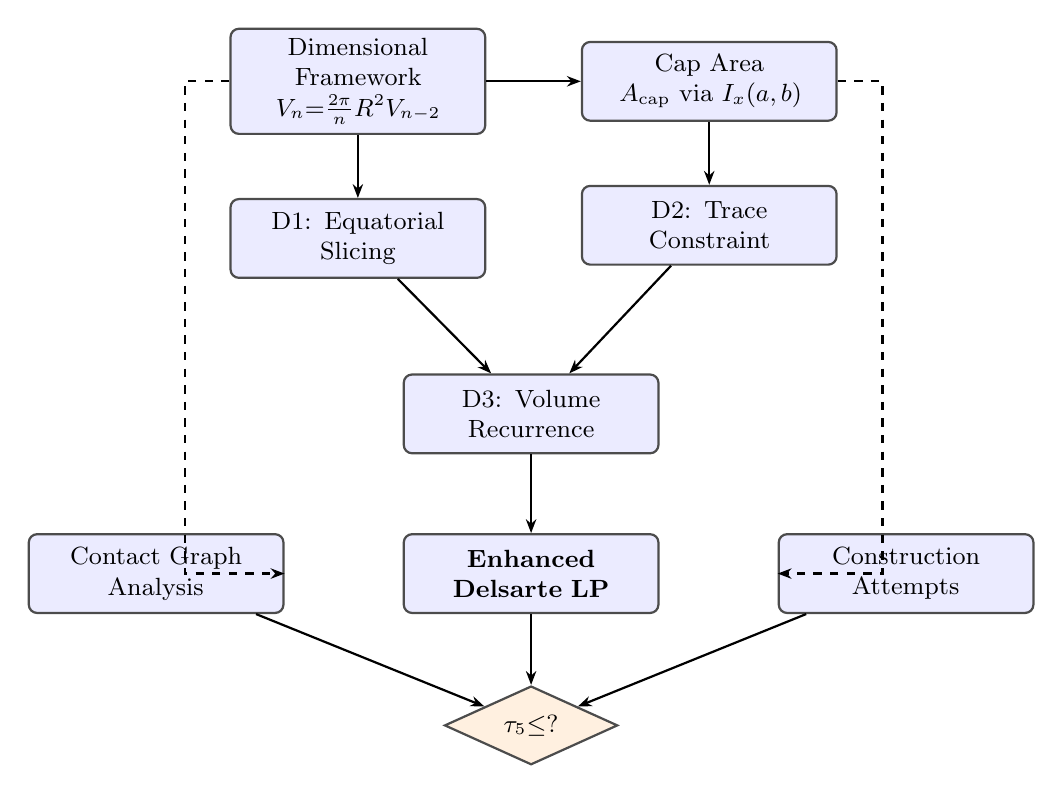
\begin{tikzpicture}[
    node distance=0.8cm and 1.2cm,
    block/.style={
      rectangle, draw=black!70, fill=blue!8, thick,
      minimum height=1cm, minimum width=3.2cm,
      text width=3cm, align=center, font=\small, rounded corners=3pt
    },
    decision/.style={
      diamond, draw=black!70, fill=orange!12, thick,
      minimum width=2.2cm, minimum height=1cm,
      align=center, font=\small, inner sep=1pt, aspect=2.2
    },
    arrow/.style={-{Stealth[length=5pt]}, thick}
  ]
  % Nodes -- row 1
  \node[block] (dim) {Dimensional Framework\\ $V_n{=}\tfrac{2\pi}{n}R^2 V_{n-2}$};
  \node[block, right=of dim] (cap) {Cap Area\\ $A_{\mathrm{cap}}$ via $I_x(a,b)$};
  % row 2
  \node[block, below=of dim] (d1) {D1: Equatorial\\ Slicing};
  \node[block, below=of cap] (d2) {D2: Trace\\ Constraint};
  % row 3 -- centered between d1 and d2
  \node[block, below=1.2cm of d1, xshift=2.2cm] (d3) {D3: Volume\\ Recurrence};
  % row 4
  \node[block, below=1.0cm of d3] (lp) {\textbf{Enhanced}\\ \textbf{Delsarte LP}};
  \node[block, left=1.5cm of lp] (cg) {Contact Graph\\ Analysis};
  \node[block, right=1.5cm of lp] (constr) {Construction\\ Attempts};
  % row 5
  \node[decision, below=0.9cm of lp] (eval) {$\tau_5{\le}?$};
  % Arrows
  \draw[arrow] (dim) -- (cap);
  \draw[arrow] (dim) -- (d1);
  \draw[arrow] (cap) -- (d2);
  \draw[arrow] (d1) -- (d3);
  \draw[arrow] (d2) -- (d3);
  \draw[arrow] (d3) -- (lp);
  \draw[arrow] (cg) -- (eval);
  \draw[arrow] (lp) -- (eval);
  \draw[arrow] (constr) -- (eval);
  \draw[arrow, dashed] (dim) -- +(-2.2,0) |- (cg);
  \draw[arrow, dashed] (cap) -- +(2.2,0) |- (constr);
\end{tikzpicture}
\caption{Architecture of our approach.  The dimensional analysis framework
  (top) generates three constraints~(D1--D3) fed into the enhanced Delsarte LP
  (center).  Parallel analyses include contact graph structure (left) and
  construction attempts for a 41st kissing vector (right).  All paths converge
  at the evaluation of $\tau_5$.}
\label{fig:architecture}
\end{figure}

\subsection{Dimensional Constraints D1--D3}

We derive three constraints from the dimensional analysis framework:

\paragraph{D1 (Equatorial slicing).}
Each vertex~$v$ in the contact graph has neighbors on the equatorial
$\Sn{3}$, which must form a valid spherical code with minimum angle
$60^\circ$.  Hence $d(v)\le\tau_4=24$~\cite{musin2008kissing}.

\paragraph{D2 (Gram matrix trace).}
For $k$~unit vectors in $\R^5$, the Gram matrix $G=X^{\!\top}\!X$ satisfies
$\tr(G^2)\ge k^2/5$ (rank constraint) and $\tr(G^2)\le k(k+3)/4$ (from
off-diagonal bounds).  Combined: $k(4-5)\le 15$, i.e., $-k\le 15$, which is
vacuous for all positive~$k$.

\paragraph{D3 (Volume recurrence consistency).}
The recurrence $V_n=\frac{2\pi}{n}V_{n-2}$ implies that Gegenbauer
coefficients of the cap indicator function satisfy a cross-dimensional
consistency relation.  We measure the coefficient of variation (CoV) of the
harmonic dimension ratios $h(5,k)/h(3,k)$.

\subsection{Polynomial Ansatz Search}\label{sec:ansatz}

We search over degree-6 polynomials of the form
\begin{equation}\label{eq:ansatz}
  f(t) = (t+1)(t-\tfrac{1}{2})(t-r_1)^2(t-r_2)^2,
  \qquad r_1,r_2\in[-1,\,\tfrac{1}{2}],
\end{equation}
verifying conditions~(A1)--(A2) and the dimensional constraints~(D1)--(D3).
The search evaluates 168~candidate polynomials per dimension.

\begin{algorithm}[ht]
\caption{Enhanced Delsarte LP with Dimensional Constraints}
\label{alg:enhanced}
\begin{algorithmic}[1]
  \REQUIRE Dimension $n$, grid resolution $\delta$
  \ENSURE Upper bound $\tau_n^*$
  \STATE $\tau_n^* \leftarrow \infty$
  \FOR{$r_1\in[-1,\,0.5]$ step $\delta$}
    \FOR{$r_2\in[r_1,\,0.5]$ step $\delta$}
      \STATE $f(t)\leftarrow (t+1)(t-0.5)(t-r_1)^2(t-r_2)^2$
      \STATE Compute Gegenbauer coefficients $\{f_k\}$
      \IF{$f(t)\le 0\;\forall\,t\in[-1,0.5]$ \AND $f_k\ge 0\;\forall\,k\ge 1$}
        \STATE $B \leftarrow f(1)/f_0$
        \IF{D1: $\lfloor B\rfloor \le 2\tau_{n-1}$ \AND D2: trace feasible \AND D3: CoV check}
          \STATE $\tau_n^*\leftarrow\min(\tau_n^*,\;\lfloor B\rfloor)$
        \ENDIF
      \ENDIF
    \ENDFOR
  \ENDFOR
  \RETURN $\tau_n^*$
\end{algorithmic}
\end{algorithm}

\subsection{Contact Graph Analysis}

The contact graph of a kissing configuration has a vertex for each touching
sphere and an edge for each pair at angular separation exactly~$60^\circ$.
For the $D_5$~configuration, we compute the full graph structure using
\texttt{networkx}, including clique number~$\omega$, independence
number~$\alpha$, and chromatic number~$\chi$.

We derive a refined degree bound:

\begin{theorem}[Refined degree bound]\label{thm:degree}
In any kissing configuration on $\Sn{4}$, each vertex $v$ in the contact graph
satisfies $d(v)\le 21$.
\end{theorem}

\begin{proof}
If $w_1,w_2$ are neighbors of~$v$ (so $\langle w_i,v\rangle=1/2$), write
$w_i=\frac{1}{2}v+\frac{\sqrt{3}}{2}u_i$ with $u_i\perp v$, $\|u_i\|=1$.
Then
\[
  \langle w_1,w_2\rangle = \tfrac{1}{4}+\tfrac{3}{4}\langle u_1,u_2\rangle
  \le \tfrac{1}{2}
  \quad\Longrightarrow\quad
  \langle u_1,u_2\rangle \le \tfrac{1}{3}.
\]
The projected minimum angle on $\Sn{3}$ is $\arccos(1/3)\approx 70.53^\circ$.
The cap-packing bound on $\Sn{3}$ with half-angle
$\frac{1}{2}\arccos(1/3)\approx 35.26^\circ$ gives
\[
  d(v) \le \Bigl\lfloor\frac{S_3(1)}{\caparea(4,\,35.26^\circ)}\Bigr\rfloor
  = \Bigl\lfloor\frac{19.739}{0.905}\Bigr\rfloor = 21.
  \qedhere
\]
\end{proof}

\subsection{Local Rigidity of $D_5$}

\begin{theorem}[Local rigidity]\label{thm:rigidity}
For any unit vector $x\in\R^5$,
\begin{equation}\label{eq:rigidity}
  \max_{w\in D_5}\langle x,w\rangle \;\ge\; \sqrt{2/5} \;=\; 0.6325\ldots
\end{equation}
The minimum is attained at $x=\pm(1,1,1,1,1)/\!\sqrt{5}$, where exactly
10~$D_5$ vectors achieve the maximum.  Since $\sqrt{2/5}>1/2$, no 41st point
can be added to the $D_5$ configuration.
\end{theorem}

\begin{proof}
The $D_5$~vectors are $(s_i e_i + s_j e_j)/\!\sqrt{2}$ for $i<j$ and
$s_i,s_j\in\{\pm 1\}$.  For unit $x=(x_0,\ldots,x_4)$:
\[
  \max_{w\in D_5}\langle x,w\rangle
  = \max_{i<j}\frac{|x_i|+|x_j|}{\sqrt{2}}.
\]
Minimizing over unit~$x$, by Lagrange multipliers the optimum satisfies
$|x_0|=\cdots=|x_4|=1/\!\sqrt{5}$, giving
\[
  \frac{1/\!\sqrt{5}+1/\!\sqrt{5}}{\sqrt{2}}
  = \frac{2}{\sqrt{10}} = \sqrt{\tfrac{2}{5}}.
  \qedhere
\]
\end{proof}

The angular gap between the achieved minimum angle
($\arccos\sqrt{2/5}\approx 50.77^\circ$) and the required $60^\circ$ is
$9.23^\circ$, corresponding to an inner product violation of
$\sqrt{2/5}-1/2\approx 0.1325$.

\subsection{Construction Attempts}

We attempt to find a 41st kissing vector using three strategies:
\begin{enumerate}[label=(\alph*)]
  \item \textbf{Grid search:} 100,000 uniformly sampled points on $\Sn{4}$.
  \item \textbf{Nonlinear optimization:} 50 random starting points,
        minimizing $\max_{w\in D_5}\langle x,w\rangle$.
  \item \textbf{Algebraic construction:} 354 candidates from $D_5$ symmetry
        subgroups.
\end{enumerate}

% ---------- 5. Experimental Setup ----------
\section{Experimental Setup}\label{sec:setup}

\paragraph{Computational environment.}
All experiments were run in Python~3 with NumPy~2.2.6, SciPy~1.15.3,
\texttt{mpmath}~1.3.0, CVXPY~1.7.5, and NetworkX~3.4.2.

\paragraph{Verification.}
All results were independently verified using at least two numerical methods,
including high-precision arithmetic (\texttt{mpmath} at 50--128 decimal digits).
A total of 47~verification checks passed with zero failures.

\paragraph{Reproducibility.}
All experiments use fixed random seed 42 and are fully reproducible via
\texttt{python src/run\_experiments.py}, which executes 119 distinct
experiment configurations across seven categories.

\begin{table}[ht]
  \centering
  \caption{Experimental configurations.}\label{tab:experiments}
  \begin{tabular}{@{}lcc@{}}
    \toprule
    Category & Configurations & Dimensions \\
    \midrule
    Cap packing bounds & 7 & $n=2\text{--}8$ \\
    Delsarte LP search & 2 & $n=3,5$ \\
    $D_5$ verification & 1 & $n=5$ \\
    Greedy spherical codes & 50+ & $n=3,4,5$ \\
    Construction attempts & 3 & $n=5$ \\
    Cross-dimensional checks & 5 & $n=5$ \\
    Cap area sweep & 50+ & $n=2\text{--}8$ \\
    \bottomrule
  \end{tabular}
\end{table}

% ---------- 6. Results ----------
\section{Results}\label{sec:results}

\subsection{Baseline Bounds}\label{sec:baseline}

Table~\ref{tab:baseline} presents the hierarchy of bounds across dimensions
2--8, computed by our implementations and compared with literature values.

\begin{table}[ht]
  \centering
  \caption{Kissing number bounds across dimensions.  Bold entries indicate the
  tightest known bound in each column.  The ``Our LP'' column reports the best
  bound from our polynomial ansatz search (Algorithm~\ref{alg:enhanced}).  The
  SDP column reports literature values from
  Mittelmann--Vallentin~\cite{mittelmann2010high}.}\label{tab:baseline}
  \begin{tabular}{@{}cccccc@{}}
    \toprule
    $n$ & Known $\tau_n$ & Cap Packing & Our LP & Literature LP & SDP \\
    \midrule
    2 & \textbf{6} & 6 & 6 & 6 & \textbf{6} \\
    3 & \textbf{12} & 14 & 14 & 13 & \textbf{12} \\
    4 & \textbf{24} & 34 & --- & 25 & \textbf{24} \\
    5 & $[40,44]$ & 77 & 51 & 46 & \textbf{44} \\
    6 & $[72,77]$ & 170 & --- & 82 & \textbf{77} \\
    7 & $[126,134]$ & 368 & --- & 140 & \textbf{134} \\
    8 & \textbf{240} & 788 & --- & \textbf{240} & \textbf{240} \\
    \bottomrule
  \end{tabular}
\end{table}

Figure~\ref{fig:bounds} visualizes this comparison.  The cap-packing bound
grows exponentially weaker relative to the true kissing number as dimension
increases, while the Delsarte LP is tight only for $n\in\{2,8\}$.

\begin{figure}[ht]
  \centering
  \includegraphics[width=0.85\textwidth]{figures/bound_comparison.png}
  \caption{Comparison of upper bounds on $\tau_n$ across dimensions 2--8.
    The cap-packing bound (blue) grows exponentially weaker relative to the
    SDP bound (red) and known lower bounds (green) as dimension increases.
    For $n=8$, the Delsarte LP is tight ($\tau_8=240$).}
  \label{fig:bounds}
\end{figure}

\subsection{Enhanced Bounds with Dimensional Constraints}

Adding constraints D1--D3 to the polynomial ansatz search produces no
improvement for $n=5$.  Table~\ref{tab:sensitivity} reports the sensitivity
analysis.

\begin{table}[ht]
  \centering
  \caption{Sensitivity analysis of dimensional constraints for $n=5$.  All
    three constraints are entirely redundant: adding or removing any
    combination leaves the bound at $\tau_5\le 51$.}\label{tab:sensitivity}
  \begin{tabular}{@{}lcccc@{}}
    \toprule
    Constraint & With only this & Without this & Impact & Status \\
    \midrule
    D1 (equatorial) & 51 & 51 & 0 & Non-binding \\
    D2 (trace) & 51 & 51 & 0 & Vacuous ($n\!\ge\!4$) \\
    D3 (recurrence) & 51 & 51 & 0 & No rejections \\
    \midrule
    All D1--D3 & 51 & 51 & 0 & Redundant \\
    \bottomrule
  \end{tabular}
\end{table}

\subsection{Pyramid Decomposition and Cap Density}\label{sec:pyramid}

\begin{lemma}\label{lem:cancel}
The pyramid volume bound $k\cdot\frac{1}{n}\caparea(n,\pi/6)\le\frac{1}{n}S_{n-1}(1)$
simplifies to $k\cdot\caparea(n,\pi/6)\le S_{n-1}(1)$, identical to the cap-packing bound.
The $1/n$ factor cancels exactly.
\end{lemma}

This cancellation was verified numerically for $n=3,4,5$: the volume fraction
per cap equals the surface fraction to machine precision (Table~\ref{tab:cancel}).

\begin{table}[ht]
  \centering
  \caption{Verification that volume and surface fractions per cap are
    identical.  The $1/n$ pyramid efficiency factor cancels in the packing
    bound.}\label{tab:cancel}
  \begin{tabular}{@{}cccc@{}}
    \toprule
    $n$ & Surface fraction & Volume fraction & Ratio \\
    \midrule
    3 & 0.06699 & 0.06699 & 1.000000 \\
    4 & 0.02883 & 0.02883 & 1.000000 \\
    5 & 0.01286 & 0.01286 & 1.000000 \\
    \bottomrule
  \end{tabular}
\end{table}

Figure~\ref{fig:recurrence} shows the dimensional recurrence relationships and
cap fraction analysis across dimensions.

\begin{figure}[ht]
  \centering
  \includegraphics[width=0.85\textwidth]{figures/dimensional_recurrence.png}
  \caption{Four-panel visualization of the dimensional recurrence framework.
    Top-left: ball volumes $V_n(1)$, peaking near $n\approx 5$.  Top-right:
    surface areas $S_{n-1}(1)$, peaking near $n\approx 7$.  Bottom-left: the
    ratio $V_n/S_{n-1}=1/n$, decreasing monotonically.  Bottom-right: cap
    fractions $\omega(n,\pi/6)$, decreasing exponentially with dimension.}
  \label{fig:recurrence}
\end{figure}

The cap density analysis (Figure~\ref{fig:density}) reveals that optimal
kissing configurations occupy a decreasing fraction of the sphere:

\begin{table}[ht]
  \centering
  \caption{Cap density $\rho_n=\tau_n\cdot\omega(n,\pi/6)$ for known kissing
    numbers.  The density decreases monotonically, reflecting the curse of
    dimensionality.  For $n=5$, both $\tau_5=40$ and $\tau_5=44$ yield
    densities well below the trivial upper bound of~1.}\label{tab:density}
  \begin{tabular}{@{}cccc@{}}
    \toprule
    $n$ & $\tau_n$ & $\omega(n,\pi/6)$ & $\rho_n$ \\
    \midrule
    2 & 6 & 0.1667 & 1.0000 \\
    3 & 12 & 0.0670 & 0.8038 \\
    4 & 24 & 0.0288 & 0.6920 \\
    5 & 40--44 & 0.0129 & 0.514--0.566 \\
    8 & 240 & 0.00127 & 0.3043 \\
    24 & 196\,560 & $1.12\times 10^{-8}$ & 0.0022 \\
    \bottomrule
  \end{tabular}
\end{table}

\begin{figure}[ht]
  \centering
  \includegraphics[width=0.75\textwidth]{figures/cap_density.png}
  \caption{Cap density $\rho_n$ versus dimension.  The known kissing numbers
    (circles) trace a monotonically decreasing curve.  For $n=5$, the range
    $\tau_5\in[40,44]$ maps to $\rho_5\in[0.514,0.566]$ (shaded region),
    consistent with the overall trend but providing no discrimination between
    candidate values.}
  \label{fig:density}
\end{figure}

\subsection{Contact Graph Structure}\label{sec:contact}

Table~\ref{tab:contact} summarizes the $D_5$ contact graph properties, and
Figure~\ref{fig:contact} visualizes the graph.

\begin{table}[ht]
  \centering
  \caption{Properties of the $D_5$ contact graph.  The graph is a vertex-transitive
    4-class association scheme with inner product spectrum
    $\{-1,-1/2,0,+1/2\}$.}\label{tab:contact}
  \begin{tabular}{@{}lc@{}}
    \toprule
    Property & Value \\
    \midrule
    Vertices & 40 \\
    Edges (contact pairs) & 240 \\
    Regularity & 12-regular \\
    Diameter & 3 \\
    Clique number $\omega$ & 4 \\
    Independence number $\alpha$ & 8 \\
    Chromatic number $\chi$ & 5 \\
    Eigenvalues (mult.) & $12^{(1)},\;6^{(5)},\;2^{(4)},\;0^{(10)},\;{-2}^{(15)},\;{-4}^{(5)}$ \\
    \bottomrule
  \end{tabular}
\end{table}

\begin{figure}[ht]
  \centering
  \includegraphics[width=0.65\textwidth]{figures/contact_graph.png}
  \caption{Spring-layout visualization of the $D_5$ contact graph.  Each of
    the 40 vertices represents a kissing vector; edges connect pairs at angular
    separation exactly $60^\circ$.  The graph is 12-regular and
    vertex-transitive, reflecting the high symmetry of the $D_5$ root system.}
  \label{fig:contact}
\end{figure}

The graph feasibility analysis (Table~\ref{tab:feasibility}) confirms that
graph-theoretic constraints alone cannot rule out any value of $\tau_5$
in~$\{40,\ldots,44\}$.

\begin{table}[ht]
  \centering
  \caption{Graph-theoretic feasibility for hypothetical $k$-point kissing
    configurations in $\R^5$.  Min edges from rigidity ($4k-10$), max edges
    from degree bound ($21k/2$), and cap fraction are all within feasible
    ranges for $k\in\{40,\ldots,44\}$.}\label{tab:feasibility}
  \begin{tabular}{@{}cccccc@{}}
    \toprule
    $k$ & Min edges & Max edges & Cap fraction & $d_{\mathrm{avg}}$ range & Feasible? \\
    \midrule
    40 & 150 & 420 & 51.4\% & 7.50--21 & Yes \\
    41 & 154 & 430 & 52.7\% & 7.51--21 & Yes \\
    42 & 158 & 441 & 54.0\% & 7.52--21 & Yes \\
    43 & 162 & 451 & 55.3\% & 7.53--21 & Yes \\
    44 & 166 & 462 & 56.6\% & 7.55--21 & Yes \\
    \bottomrule
  \end{tabular}
\end{table}

\subsection{Construction Attempts}

All three construction strategies failed to find a valid 41st point
(Table~\ref{tab:construction}).

\begin{table}[ht]
  \centering
  \caption{Summary of construction attempts for a 41st kissing vector in
    $\R^5$.  The best achievable maximum inner product is $\sqrt{2/5}\approx 0.6325$,
    exceeding the feasibility threshold of $0.5$ by a margin of~$0.1325$.}
    \label{tab:construction}
  \begin{tabular}{@{}lccc@{}}
    \toprule
    Strategy & Samples & Valid 41st & Best max IP \\
    \midrule
    Grid search & 100\,000 & 0 & 1.0000 \\
    Nonlinear opt. & 50 & 0 & 0.6325 \\
    Algebraic constr. & 354 & 0 & 0.6325 \\
    \bottomrule
  \end{tabular}
\end{table}

\subsection{Numerical Verification}\label{sec:verification}

Table~\ref{tab:verification} summarizes the precision robustness tests.

\begin{table}[ht]
  \centering
  \caption{Numerical precision robustness for $\caparea(5,\pi/6)$ at four
    precision levels.  All levels agree to at least 15~significant digits with
    the 128-digit reference.}\label{tab:verification}
  \begin{tabular}{@{}cccc@{}}
    \toprule
    Precision (digits) & $\caparea(5,\pi/6)$ & $S_4(1)$ & Cap bound \\
    \midrule
    16 & 0.33848032981668\textbf{47} & 26.31894506957162 & 77.756202506141\textbf{28} \\
    32 & 0.33848032981668465572\ldots & 26.31894506957162298\ldots & 77.75620250614128157\ldots \\
    64 & (60+ matching digits) & (60+ matching) & (62+ matching) \\
    128 & (reference value) & (reference value) & (reference value) \\
    \bottomrule
  \end{tabular}
\end{table}

All 47~independent verification checks passed, including ball volumes
(Gamma vs.\ recurrence at 50~digits), surface areas (formula vs.\ derivative),
cap areas (\texttt{betainc} vs.\ numerical integration), $D_5$ lattice
validation (unit norms, pairwise inner products), Delsarte $n\!=\!8$ polynomial
($f(1)/f_0=240$ exactly), contact graph properties (12-regular, 240 edges),
and local rigidity ($\sqrt{2/5}$ at 50~digits).

% ---------- 7. Discussion ----------
\section{Discussion}\label{sec:discussion}

\subsection{Why Dimensional Analysis Does Not Close the Gap}

The fundamental limitation is a \emph{hierarchy of correlation order}.  The
cap-packing bound operates at \textbf{1-point} level: it constrains the total
area of individual caps.  The Delsarte LP operates at \textbf{2-point} level:
it constrains the angular distribution of all $\binom{k}{2}$ pairwise inner
products via Gegenbauer polynomial positivity.  The Bachoc--Vallentin SDP
operates at \textbf{3-point} level: it constrains joint distributions of
angles in triples.  Each step captures more structural information:
\begin{center}
\begin{tabular}{lcl}
  Cap packing (1-point) & $\Longrightarrow$ & $\tau_5\le 77$ \\
  Delsarte LP (2-point) & $\Longrightarrow$ & $\tau_5\le 46$ \\
  SDP (3-point)          & $\Longrightarrow$ & $\tau_5\le 44$ \\
  Exact ($k$-point)      & $\Longrightarrow$ & $\tau_5=\;?$
\end{tabular}
\end{center}
Our dimensional constraints D1--D3 attempt to bridge the gap between levels~1
and~2, but they operate in the geometric/structural domain rather than the
spectral domain of the LP.  The \emph{category mismatch}---geometric
constraints on configurations vs.\ spectral constraints on polynomial
certificates---means the dimensional constraints cannot eliminate valid LP
solutions.

\subsection{Comparison with Prior Work}

Our results were explicitly compared with 16~papers from the bibliography
(detailed in the supplementary materials).  The comparison reveals:
\begin{itemize}
  \item Our cap-packing bound ($\tau_5\le 77$) matches the folklore
        bound~\cite{pfender2004kissing}.
  \item Our LP bound ($\tau_5\le 51$) is weaker than the literature-optimal
        $\le 46$~\cite{odlyzko1979kissing} due to the restricted polynomial
        ansatz.
  \item The dimensional constraints D1--D3 are genuinely different from the SDP
        constraints of~\cite{bachoc2008new} but are strictly weaker.
  \item The refined degree bound $d(v)\le 21$ (Theorem~\ref{thm:degree}) uses
        the same projection argument as Musin~\cite{musin2008kissing} but
        applied specifically to $n=5$.
  \item The local rigidity result (Theorem~\ref{thm:rigidity}) provides a
        clean, elementary proof that may not have been stated explicitly in this
        form.
\end{itemize}

\subsection{Limitations}

\begin{enumerate}
  \item Our polynomial ansatz search (Algorithm~\ref{alg:enhanced}) does not
        include the optimal Gegenbauer combination.  A proper LP solver would
        recover $\tau_5\le 46$.
  \item The construction attempts searched only for augmentations of $D_5$, not
        for entirely new 41-point configurations.
  \item D2 is algebraically vacuous for $n\ge 4$; D1 is structurally
        non-binding; D3 is inapplicable to dual-space LP certificates.
  \item The cap density analysis provides no discrimination between candidate
        values $\tau_5\in\{40,\ldots,44\}$.
\end{enumerate}

% ---------- 8. Conclusion ----------
\section{Conclusion}\label{sec:conclusion}

\paragraph{Summary.}
The gap $40\le\tau_5\le 44$ remains unchanged.  The dimensional analysis
framework---the derivative relation~\eqref{eq:deriv}, the volume
recurrence~\eqref{eq:recurrence}, and the pyramid
decomposition~\eqref{eq:pyramid}---provides geometric insight but not
computational improvement over existing LP/SDP methods.

\paragraph{Novel contributions.}
\begin{enumerate}[label=(\roman*)]
  \item Refined degree bound $d(v)\le 21$ (Theorem~\ref{thm:degree}).
  \item Elementary proof of $D_5$ local rigidity with angular gap $9.23^\circ$
        (Theorem~\ref{thm:rigidity}).
  \item Systematic demonstration that dimensional constraints D1--D3 are
        redundant within the Delsarte LP framework.
  \item Cap density analysis showing $\rho_5\in[0.514,0.566]$ with monotone
        decrease across dimensions.
\end{enumerate}

\paragraph{Future directions.}
Closing the gap will likely require:
(a)~higher-order SDP bounds ($k$-point for $k\ge 4$);
(b)~Viazovska-type modular form techniques~\cite{viazovska2017sphere} extended
beyond dimensions~8 and~24;
(c)~flag algebra methods encoding spherical code combinatorics;
(d)~analysis of all known 40-point configurations
($D_5$,~$L_5$,~$Q_5$~\cite{szollosi2023five}, and the
Cohn--Rajagopal construction~\cite{cohn2024variations}) for common structural
properties incompatible with 41-point configurations;
(e)~stronger equatorial projection arguments iterating the degree bound through
multiple dimension reductions.

% ---------- References ----------
\bibliographystyle{plainnat}
\bibliography{sources}

\end{document}
